\section{Ứng dụng phân tích mã nguồn có lỗ hổng bảo mật}

Tính đến năm 2023, tổng cộng có 17 thể loại bug được báo cáo về RUSTSEC Database \cite{zheng2023closer}.
Trong đó, lỗi về an toàn bộ nhớ và đa luồng chiếm tới gần hai phần ba tổng số loại lỗi.
Mặc dù Rust có các cơ chế để khắc phục những lỗi này, nhưng dường như trong những dự án thực tế phức tạp, vẫn tồn tại một số lỗi nhất định, đặc biệt khi sử dụng tính năng \texttt{unsafe} (mã không an toàn) của Rust.
Để minh họa cho việc áp dụng đồ thị CPG vào thực tế, khóa luận sẽ trình bày ứng dụng của đồ thị CPG trên 4 lỗi trong RUSTSEC Database thuộc các thể loại lỗi phổ biến nhất.

\subsection{RUSTSEC-2021-0086}

% Đoạn mã \ref{code:c4_RUSTSEC-2021-0086} minh họa một lỗ hổng bảo mật phổ biến liên quan đến việc khởi tạo bộ nhớ không an toàn trong Rust. Lỗi xảy ra khi sử dụng hàm \texttt{Vec::with_capacity} để tạo một vectơ có dung lượng dự kiến, sau đó tùy ý điều chỉnh độ dài của vectơ bằng hàm \texttt{set_len}. Tuy nhiên, hàm \texttt{set_len}, một hàm không an toàn, chỉ đơn thuần thay đổi kích thước của vectơ mà không khởi tạo giá trị cho các phần tử mới được thêm vào. Điều này dẫn đến tình trạng các phần tử này chứa giá trị rác, tiềm ẩn nhiều nguy cơ như lỗi tràn bộ nhớ, truy cập trái phép vào vùng nhớ và các vấn đề bảo mật nghiêm trọng khác.

% Để khắc phục lỗi này, Rust cung cấp macro \texttt{vec!} giúp khởi tạo vectơ một cách an toàn hơn. Khi sử dụng macro này, chúng ta có thể chỉ định rõ độ dài và giá trị ban đầu cho các phần tử của vectơ, đảm bảo rằng tất cả các phần tử đều được khởi tạo với giá trị mong muốn. Trong Hình \ref{img:c4_RUSTSEC-2021-0086}, nút \texttt{BLOCK} với thuộc tính \texttt{unsafe} đánh dấu rõ ràng vùng mã không an toàn, trong khi các nút con của nó thể hiện các hoạt động cụ thể có khả năng gây ra lỗi.

Đoạn mã \ref{code:c4_RUSTSEC-2021-0086} minh họa một lỗ hổng bảo mật phổ biến liên quan đến việc khởi tạo bộ nhớ không an toàn trong Rust.
Lỗi xảy ra khi sử dụng hàm \texttt{Vec::with\_capacity} để tạo một vectơ có dung lượng được định sẵn là $N$, sau đó tùy chỉnh độ dài của vectơ bằng hàm \texttt{set\_len}.
Tuy nhiên hàm \texttt{set\_len}, một hàm được coi là \texttt{"unsafe"}, chỉ đơn thuần thay đổi kích thước của vectơ mà không khởi tạo giá trị cho các phần tử mới được thêm vào.
Điều này dẫn đến tình trạng các phần tử này chứa giá trị rác, tiềm ẩn nhiều nguy cơ như lỗi tràn bộ nhớ, truy cập trái phép vào vùng nhớ và các vấn đề bảo mật nghiêm trọng khác.
Để sửa lỗi, ta có thể sử dụng macro \texttt{vec!} để khởi tạo vectơ với độ dài và dung lượng là $N$, giá trị mặc định của mỗi phần tử là $0$.
% Trong Hình \ref{img:c4_RUSTSEC-2021-0086}, nút \texttt{BLOCK} với thuộc tính \texttt{unsafe} biểu diễn việc bắt đầu một khối lệnh không an toàn.
Trong Hình \ref{img:c4_RUSTSEC-2021-0086}, nút \texttt{BLOCK} với thuộc tính \texttt{unsafe} đánh dấu rõ ràng vùng mã không an toàn.
Các nút con của nút \texttt{BLOCK} này biểu diễn các mệnh đề, lời gọi hàm không an toàn.

\begin{listing}[H]
\begin{minted}[mathescape, breaklines, frame=lines, framesep=2mm, baselinestretch=1.2, fontsize=\footnotesize, linenos]{rust}
// Before fix
let mut buf: Vec<u8> = Vec::with_capacity(N);
unsafe { buf.set_len(N) };
// After fix
let mut buf: Vec<u8> = vec![0; N];
\end{minted}
\caption{Ví dụ đoạn mã nguồn cho RUSTSEC-2021-0086.}
\label{code:c4_RUSTSEC-2021-0086}
\end{listing}

\begin{figure}[H]
    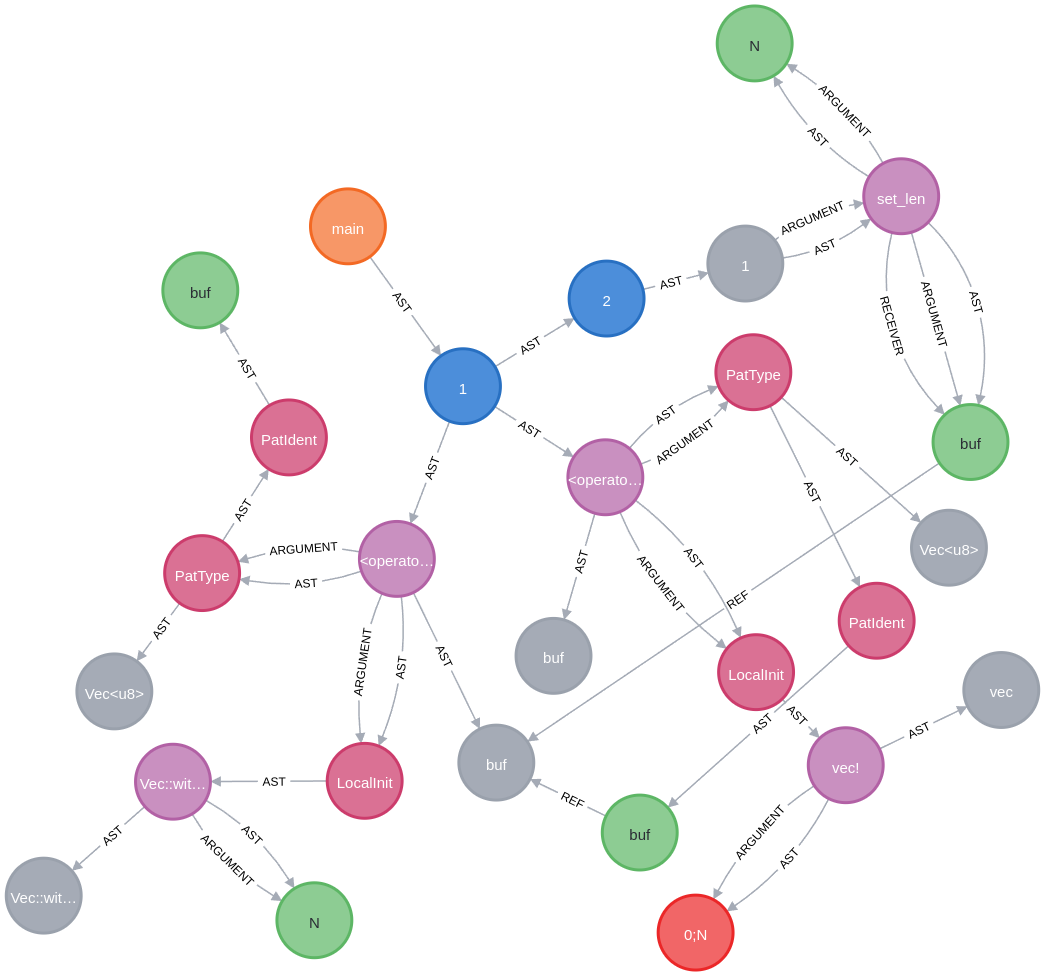
\includegraphics[width=1\columnwidth]{figures/c4/c4_RUSTSEC-2021-0086.png}
    \centering
    \caption{Minh họa đồ thị CPG cho đoạn mã nguồn RUSTSEC-2021-0086 \ref{code:c4_RUSTSEC-2021-0086}.}
    \label{img:c4_RUSTSEC-2021-0086}
\end{figure}

\subsection{RUSTSEC-2022-0028}

\begin{listing}[H]
\begin{minted}[mathescape, breaklines, frame=lines, framesep=2mm, baselinestretch=1.2, fontsize=\footnotesize, linenos]{rust}
// Before fix
pub fn external<'a, T>(data: T) -> Handle<'a, Self>
where
    T: AsMut<[u8]> + Send,
{
    // ...
}

// After fix
pub fn external<'a, T>(data: T) -> Handle<'a, Self>
where
    T: AsMut<[u8]> + Send + 'static,
{
    // ...
}
\end{minted}
\caption{Ví dụ đoạn mã nguồn cho RUSTSEC-2022-0028.}
\label{code:c4_RUSTSEC-2022-0028}
\end{listing}

Đoạn mã \ref{code:c4_RUSTSEC-2022-0028} mô tả lỗi xảy ra khi sử dụng hàm \texttt{external} mà không xác định đúng ràng buộc lifetime cho kiểu tổng quát \texttt{T}.
Trong bối cảnh này, \texttt{external} là hàm được dùng để tạo ra dữ liệu giao tiếp chung giữa Rust và Javascript thông qua Web Assembly Binding \cite{ githubGitHubRustwasmwasmbindgen}.
Việc kiểu tổng quát \texttt{T} không được xác định đúng lifetime cho phép tạo ra một vùng dữ liệu có thể bị giải phóng trong khi chúng vẫn được tham chiếu bởi mã nguồn Javascript.
Để hai ngôn ngữ có thể giao tiếp được thì dữ liệu đó phải tồn tại trong suốt thời gian chạy của cả hai ngôn ngữ.
Để sửa lỗi, cần thêm ràng buộc \texttt{T: 'static} để đảm bảo rằng dữ liệu được tham chiếu sẽ không bị giải phóng trong suốt thời gian tồn tại của chương trình.
RUSTSEC-2022-0028 là một lỗi thực sự rất khó để phát hiện tự động vì nó liên quan đến bối cảnh mã nguồn, ở đây là dữ liệu giao tiếp giữa 2 ngôn ngữ Rust và Javascript thông qua Web Assembly Binding.
Nếu chỉ sử dụng các mẫu khai phá tự động thông thường trên đồ thị CPG để phân tích thì chưa chắc phát hiện ra lỗi.
Do cần kiến thức về bối cảnh bài toán nên sự can thiệp của con người là cần thiết trong trường hợp này.
Trong Hình \ref{img:c4_RUSTSEC-2022-0028}, các câu truy vấn trên đồ thị CPG kết hợp với kiến thức miền của các chuyên gia cần được xây dựng thủ công để có thể phát hiện ra lỗ hổng.
% Hình \ref{img:c4_RUSTSEC-2022-0028} cũng thể chưa trình bày một cách rõ ràng lỗi có thể xảy ra khi sử dụng hàm \texttt{external} và kiểu tổng quát \texttt{T}, do cần đến bối cảnh bài toán.

% \begin{listing}[H]
% \begin{minted}[mathescape, breaklines, frame=lines, framesep=2mm, baselinestretch=1.2, fontsize=\footnotesize, linenos]{rust}
% // Before fix
% pub fn external<'a, C, T>(cx: &mut C, data: T) -> Handle<'a, Self>
% where
%     C: Context<'a>,
%     T: AsMut<[u8]> + Send,
% {
%     // ...
% }

% // After fix
% pub fn external<'a, C, T>(cx: &mut C, data: T) -> Handle<'a, Self>
% where
%     C: Context<'a>,
%     T: AsMut<[u8]> + Send + 'static,
% {
%     // ...
% }
% \end{minted}
% \caption{Ví dụ đoạn mã nguồn cho RUSTSEC-2022-0028}
% \label{code:c4_RUSTSEC-2022-0028}
% \end{listing}


\begin{figure}[H]
    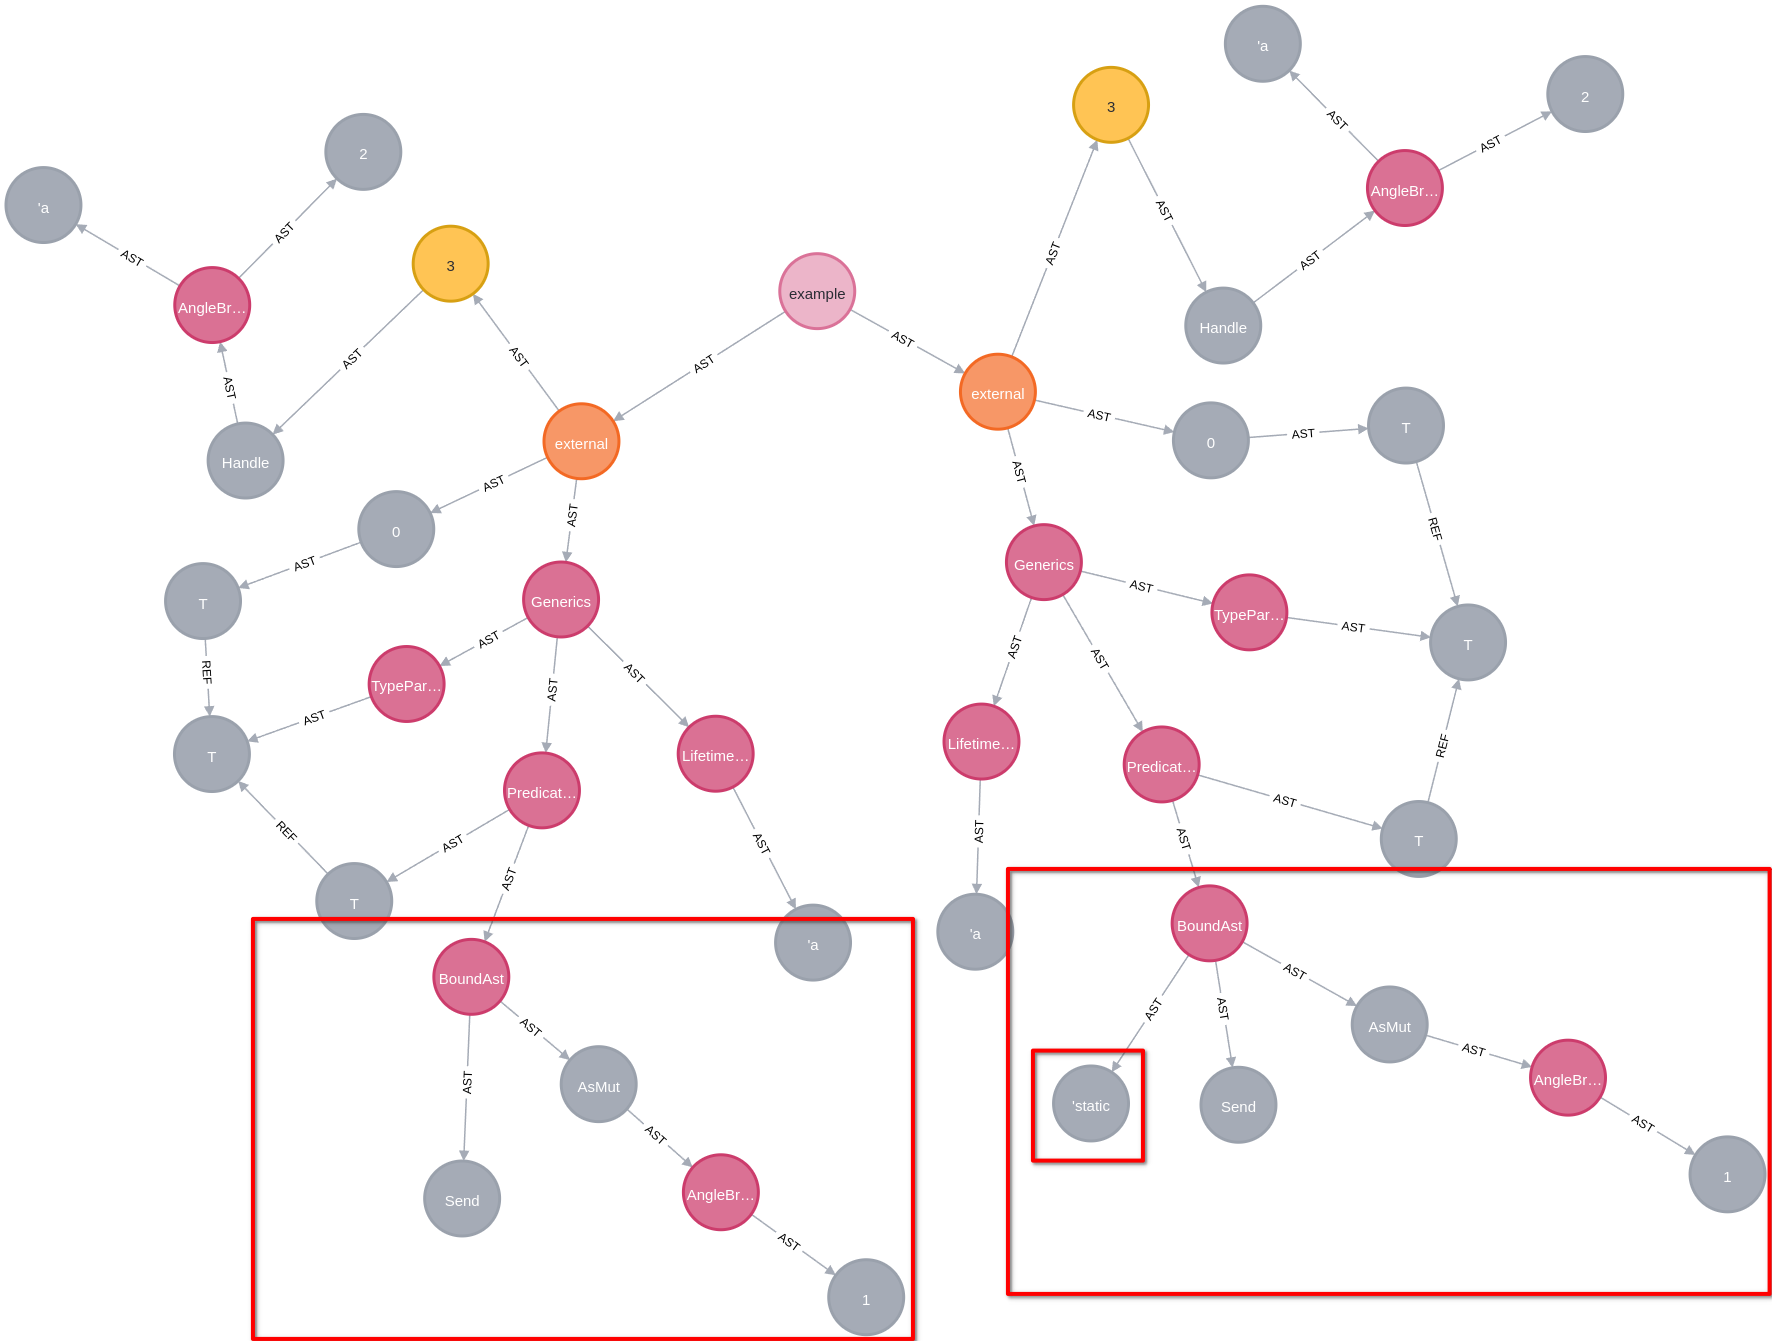
\includegraphics[width=1\columnwidth]{figures/c4/c4_RUSTSEC-2022-0028.png}
    \centering
    \caption{Minh họa đồ thị CPG cho đoạn mã nguồn RUSTSEC-2022-0028 \ref{code:c4_RUSTSEC-2022-0028}.}
    \label{img:c4_RUSTSEC-2022-0028}
\end{figure}


\subsection{RUSTSEC-2020-0044}


\begin{listing}[H]
\begin{minted}[mathescape, breaklines, frame=lines, framesep=2mm, baselinestretch=1.2, fontsize=\footnotesize, linenos]{rust}
// Before fix
unsafe impl<P> Send for Atom<P> where P: IntoRawPtr + FromRawPtr {}
unsafe impl<P> Sync for Atom<P> where P: IntoRawPtr + FromRawPtr {}

// After fix
unsafe impl<P> Send for Atom<P> where P: IntoRawPtr + FromRawPtr + Send {}
unsafe impl<P> Sync for Atom<P> where P: IntoRawPtr + FromRawPtr + Sync {}
\end{minted}
\caption{Ví dụ đoạn mã nguồn cho RUSTSEC-2020-0044.}
\label{code:c4_RUSTSEC-2020-0044}
\end{listing}

Đoạn mã \ref{code:c4_RUSTSEC-2020-0044} mô tả lỗi liên quan đến việc không triển khai thuộc tính \texttt{Send} và \texttt{Sync} cho kiểu dữ liệu con bên trong kiểu \texttt{Atom}.
Trong bối cảnh này, \texttt{Atom} đóng vai trò như một hộp chứa cho kiểu dữ liệu \texttt{P} bên trong, giúp quản lý việc sử dụng bộ nhớ an toàn hơn.
Tuy nhiên chỉ mình \texttt{Atom} được cài đặt thuộc tính \texttt{Send} và \texttt{Sync}, không đảm bảo rằng kiểu dữ liệu con \texttt{P} cũng phải cài đặt thuộc tính \texttt{Send} và \texttt{Sync}.
Điều này có nghĩa việc truy cập đến \texttt{Atom} có thể an toàn nhưng khi truy cập vào dữ liệu kiểu \texttt{P} bên trong thì không an toàn, có thể dẫn đến các vấn đề như sử dụng bộ nhớ sau khi đã giải phóng hoặc tương tranh dữ liệu cho kiểu dữ liệu \texttt{P} bên trong.
Để sửa lỗi này, cần đảm bảo rằng kiểu \texttt{P} cũng phải được đánh dấu thuộc tính \texttt{Send} và \texttt{Sync}.

\begin{figure}[H]
    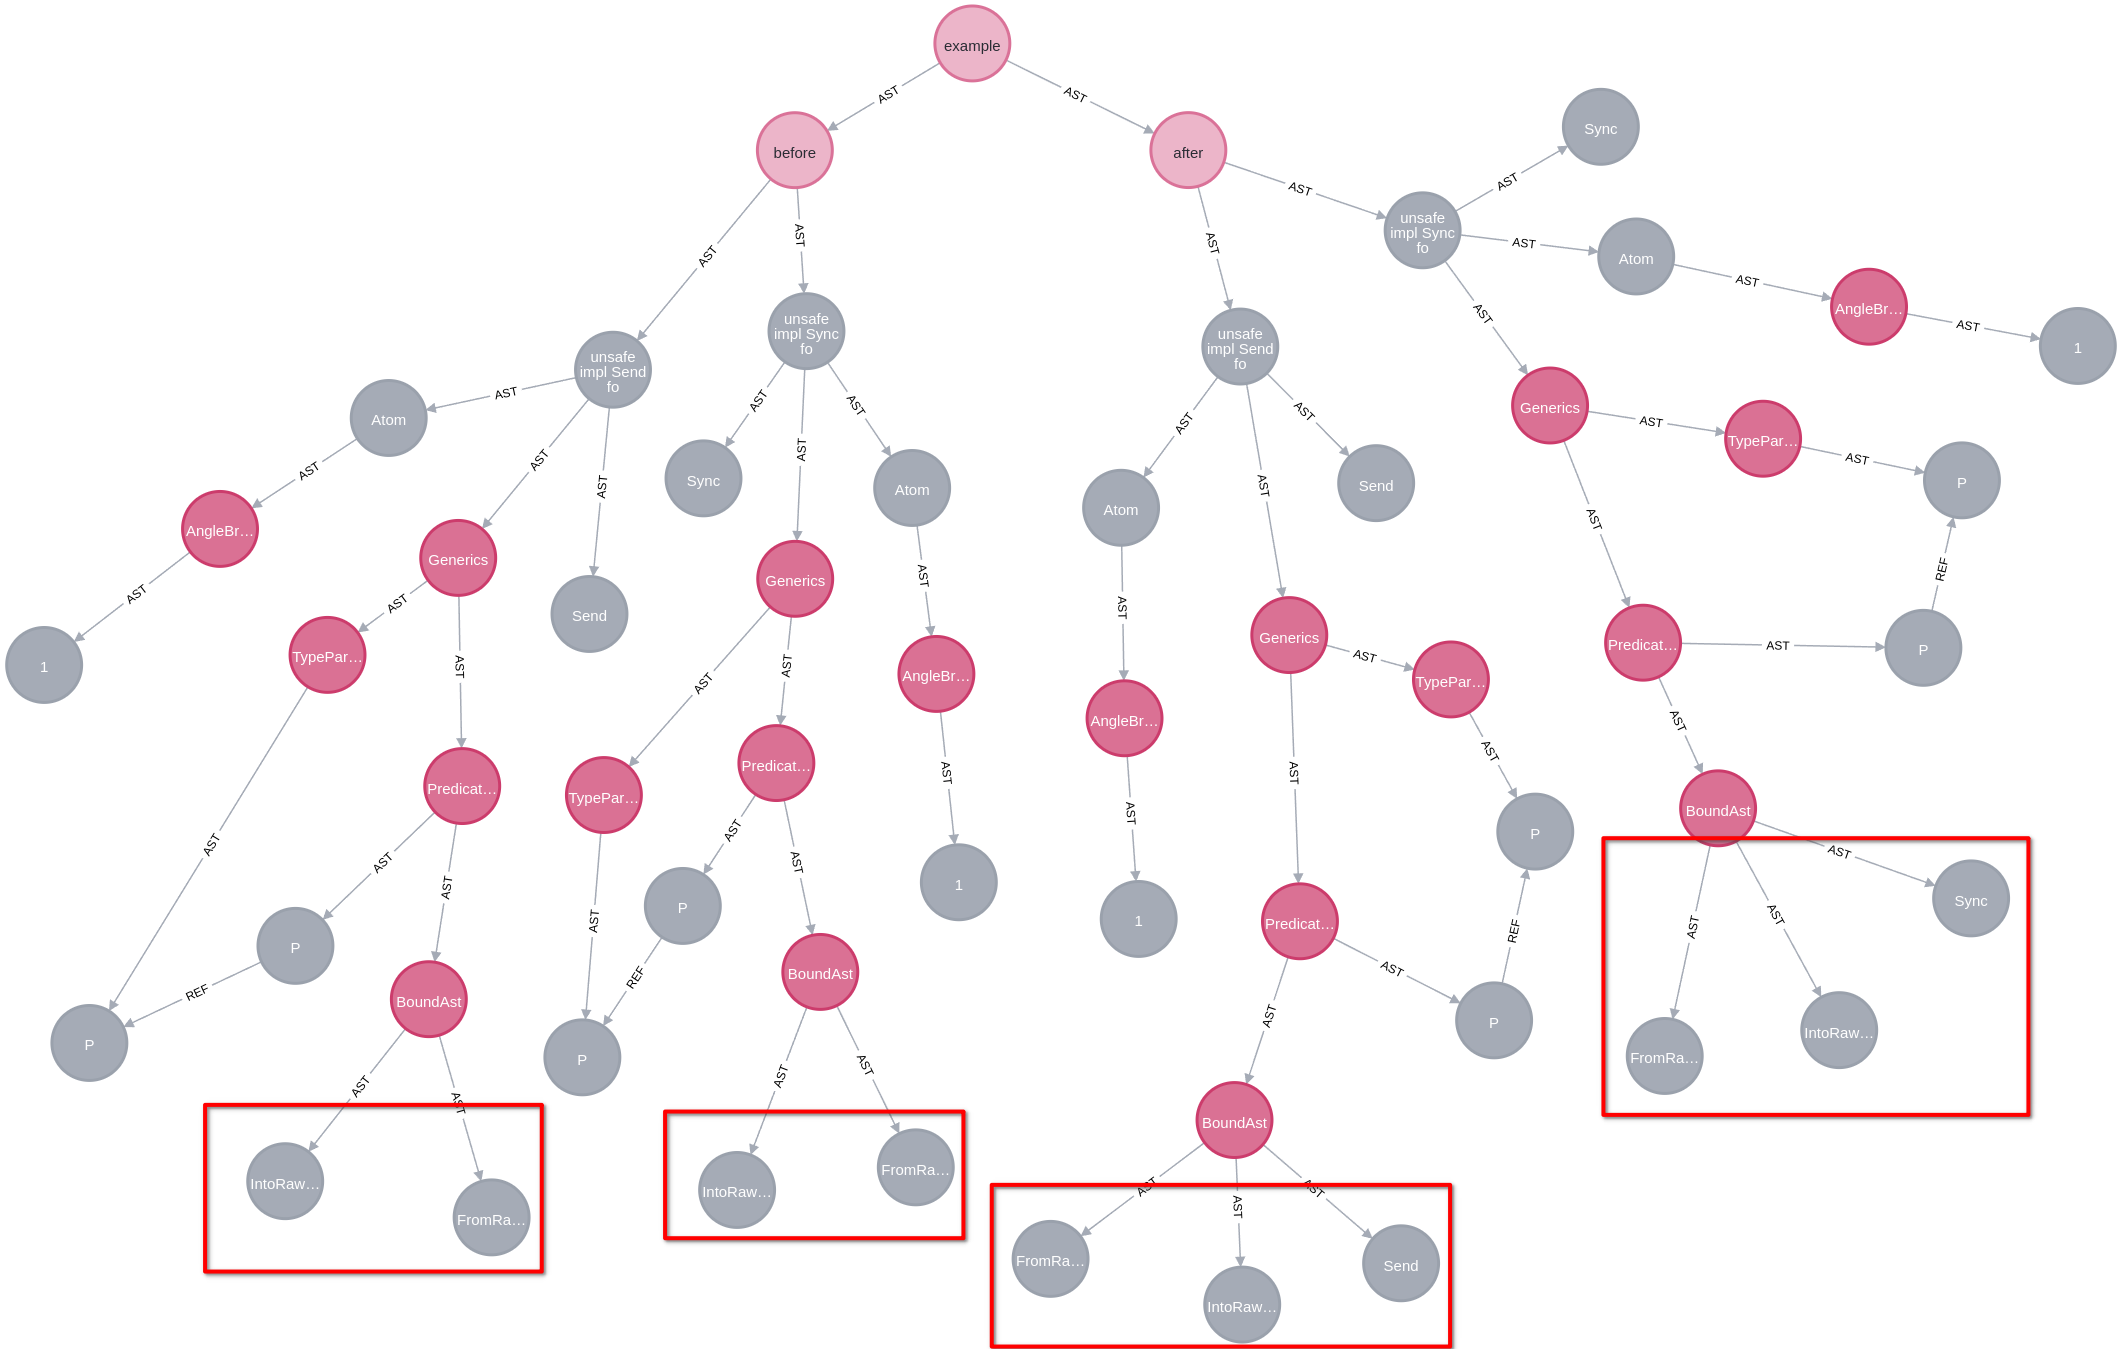
\includegraphics[width=1\columnwidth]{figures/c4/c4_RUSTSEC-2020-0044.png}
    \centering
    \caption{Minh họa đồ thị CPG cho đoạn mã nguồn RUSTSEC-2020-0044 \ref{code:c4_RUSTSEC-2020-0044}.}
    \label{img:c4_RUSTSEC-2020-0044}
\end{figure}

Lỗi RUSTSEC-2020-0044 là một lỗi xảy ra thường xuyên khi lập trình đa luồng trong Rust.
Kiểu cha muốn đảm bảo an toàn về đa luồng thì kiểu con cũng phải đảm bảo an toàn về đa luồng.
Trong bối cảnh của Rust, điều này có nghĩa là nếu kiểu cha muốn được gửi qua các luồng một cách an toàn bằng thuộc tính \texttt{Send} và \texttt{Sync} thì kiểu con cũng phải có khả năng này.
Khi được biểu diễn trực quan trên Hình \ref{code:c4_RUSTSEC-2020-0044}, hoàn toàn ta có thể thấy một mẫu duyệt đồ thị để phát hiện lỗi này.
Một mẫu khai phá đồ thị phổ biến có thể được xây dựng và sử dụng cho nhiều đoạn mã khác nhau.
Các truy vấn hoặc phân tích dựa trên mẫu này có thể được áp dụng trên đồ thị CPG để phát hiện các lỗi tương tự.

\subsection{RUSTSEC-2021-0130}

\begin{listing}[H]
\begin{minted}[mathescape, breaklines, frame=lines, framesep=2mm, baselinestretch=1.2, fontsize=\footnotesize, linenos]{rust}
// Before fix
pub fn iter<'a>(&'_ self) -> Iter<'a, K, V> {
    Iter { ptr: unsafe { (*self.head).next }, }
}
// After fix
pub fn iter(&self) -> Iter<'_, K, V> {
    Iter { ptr: unsafe { (*self.head).next }, }
}
\end{minted}
\caption{Ví dụ đoạn mã nguồn cho RUSTSEC-2021-0130.}
\label{code:c4_RUSTSEC-2021-0130}
\end{listing}

Đoạn mã \ref{code:c4_RUSTSEC-2021-0130} mô tả về một lỗi sử dụng bộ nhớ sau khi đã giải phóng.
Trong bối cảnh này, \texttt{Iter} là một \texttt{struct} được sử dụng để duyệt qua các phần tử trong một danh sách liên kết.
Tuy nhiên, khi \texttt{Iter} được trả về từ hàm \texttt{iter} thì nó sẽ trỏ tới \texttt{self.head} mà \texttt{self.head} có thể bị giải phóng trước khi \texttt{Iter} được sử dụng, dẫn đến việc sử dụng bộ nhớ sau khi đã giải phóng.
Nguyên nhân là do quan hệ lifetime giữa biến \texttt{self} và giá trị trả về kiểu \texttt{Iter} không đồng bộ.
Biến \texttt{self} được chỉ định lifetime là \texttt{'\_}, tức là để trình biên dịch tự động gán một giá trị lifetime mặc định, trong khi đó kiểu trả về \texttt{Iter} được chỉ định lifetime là \texttt{'a}.
Trong trường hợp này \texttt{'\_} và \texttt{'a} không có liên hệ với nhau do đó lifetime của \texttt{Iter} có thể lớn hơn lifetime của \texttt{self}, dẫn đến việc truy cập đến \texttt{self.head} sau khi \texttt{self} đã bị giải phóng.
Để sửa lỗi, cần sử dụng chung một lifetime cho \texttt{self} và \texttt{Iter} thông qua việc sử dụng 3 quy tắc lược bỏ lifetime \cite{rustlangLifetimeElision}.
Nếu không chỉ định lifetime một cách tường minh, ba quy tắc lược bỏ lifetime sẽ được trình biên dịch sử dụng để tự động xác định lifetime của các biến dựa trên cấu trúc của hàm, bao gồm:

\begin{enumerate}
    \item Mỗi tham số kiểu tham chiếu của hàm mặc định có một lifetime riêng.
    \item Khi hàm có một tham số kiểu tham chiếu duy nhất, và kiểu trả về cũng là kiểu tham chiếu thì lifetime của kiểu trả về sẽ là lifetime của tham số tham số kiểu tham chiếu duy nhất đó.
    \item Nếu hàm có nhiều tham số kiểu tham chiếu nhưng có một tham số là \texttt{self} (\texttt{self} tương đương với \texttt{this} trong C++ và Java), thì lifetime của \texttt{self} sẽ được gán cho kiểu tham số trả về.
\end{enumerate}

Trong trường hợp này, ta sửa lỗi bằng cách không chỉ định lifetime cho \texttt{self} mà để trình biên dịch tự xác định, lifetime của \texttt{Iter} sẽ để là \texttt{'\_}.
Ký hiệu \texttt{'\_} tức là tự động suy diễn và áp dụng quy tắc số 3 thì lifetime của \texttt{Iter} sẽ được gán bằng lifetime của \texttt{self}.
Từ đó lifetime của \texttt{Iter} sẽ không lớn hơn lifetime của \texttt{self} và việc truy cập đến \texttt{self.head} sau khi \texttt{self} đã bị giải phóng sẽ không xảy ra.

\begin{figure}[H]
    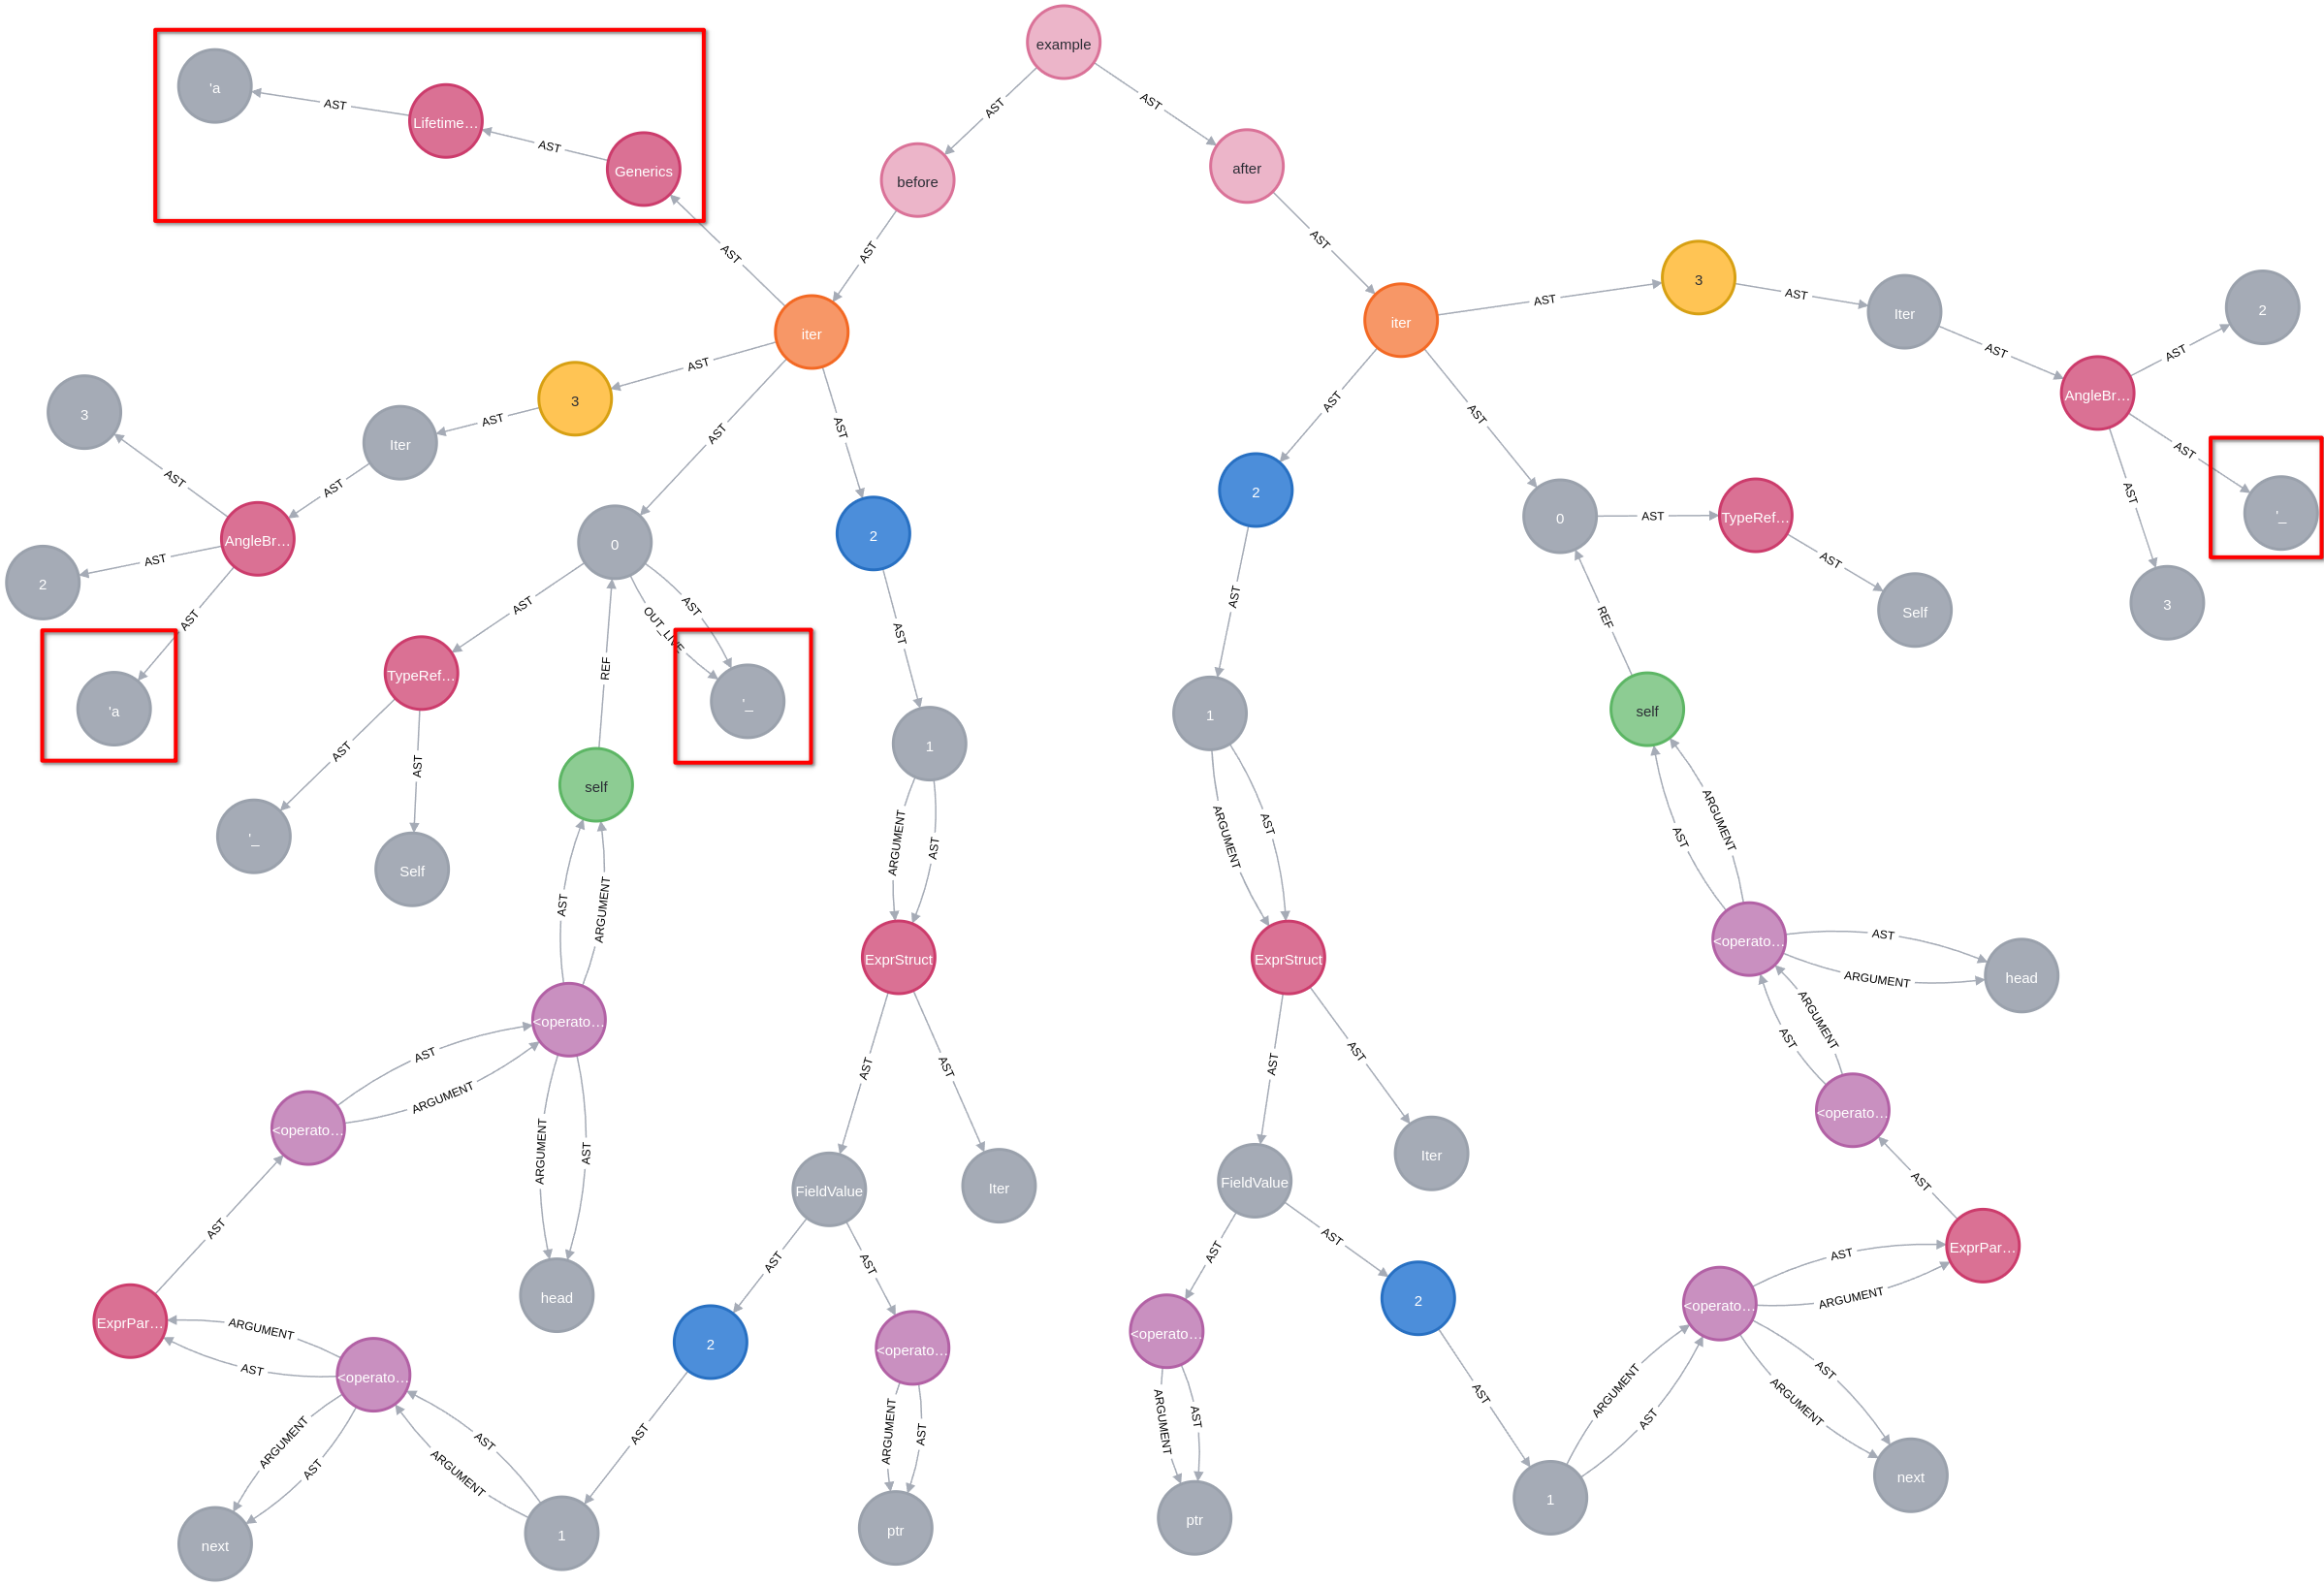
\includegraphics[width=1\columnwidth]{figures/c4/c4_RUSTSEC-2021-0130.png}
    \centering
    \caption{Minh họa đồ thị CPG cho đoạn mã nguồn RUSTSEC-2021-0130 \ref{code:c4_RUSTSEC-2021-0130}.}
    \label{img:c4_RUSTSEC-2021-0130}
\end{figure}

Đánh dấu lifetime một cách tường minh cần được thực hiện cẩn thận để tránh được các lỗi liên quan đến bộ nhớ.
Việc đánh dấu lifetime không chính xác có thể đánh lừa trình biên dịch và dẫn đến việc sử dụng bộ nhớ sau khi đã giải phóng.
Lifetime của kiểu trả về phải đảm bảo không lớn hơn lifetime của tham số truyền vào nếu kiểu trả về có truy cập đến bộ nhớ của tham số truyền vào.
Có thể áp dụng ba quy tắc lược bỏ lifetime để suy diễn việc xác định lifetime giữa tham số và tham số, giữa tham số và kiểu trả về.
Kết hợp với đồ thị CPG \ref{img:c4_RUSTSEC-2021-0130}, các luật có thể được đề ra để phát hiện sự không đồng bộ về lifetime giữa các biến dựa vào các nút \texttt{LIFETIME},
\texttt{LIFETIME PARAMETER} và các cạnh thể hiện mối quan hệ giữa chúng như , \texttt{REF}, \texttt{OUT LIVE}.
